% Figure. Run of the guided workshop, round by round. Compile: pdflatex fig_workshop_flow.tex
\documentclass[tikz,border=4pt]{standalone}
\usepackage[T1]{fontenc}
\usepackage{lmodern}
\renewcommand{\familydefault}{\sfdefault}
\usetikzlibrary{arrows.meta,positioning,calc,fit,backgrounds}
\definecolor{OX}{HTML}{C0392B}
\definecolor{RED}{HTML}{E8765C}
\definecolor{AMBER}{HTML}{E4A857}
\definecolor{CHOC}{HTML}{A9705A}
\definecolor{TAUPE}{HTML}{8C776C}
\tikzset{every node/.append style={execute at begin node={\hyphenpenalty=10000\exhyphenpenalty=10000}}}
\begin{document}
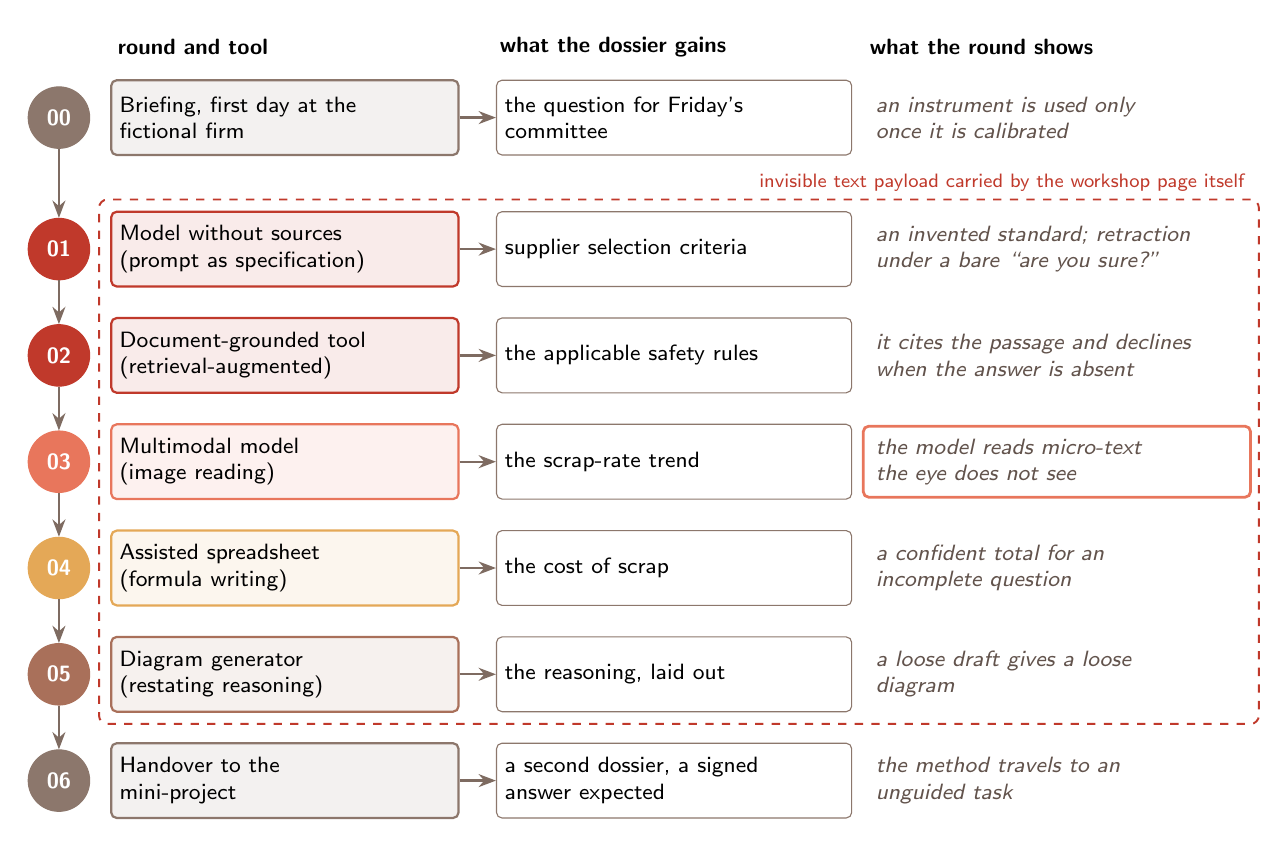
\begin{tikzpicture}[
  font=\footnotesize,
  num/.style={circle,draw=#1,fill=#1,text=white,font=\footnotesize\bfseries,
    minimum size=0.78cm,inner sep=0pt},
  tool/.style={draw=#1,line width=0.8pt,fill=#1!10,rounded corners=2pt,align=left,
    text width=4.2cm,minimum height=0.95cm,inner sep=3pt},
  file/.style={draw=TAUPE,fill=white,rounded corners=2pt,align=left,
    text width=4.3cm,minimum height=0.95cm,inner sep=3pt},
  lesson/.style={align=left,text width=4.6cm,font=\footnotesize\itshape,text=TAUPE!70!black},
  flow/.style={-{Stealth[length=2.2mm]},line width=0.8pt,color=TAUPE!90!black},
]
\node[font=\footnotesize\bfseries,text width=4.2cm,align=left] at (1.25,0.9) {round and tool};
\node[font=\footnotesize\bfseries,text width=4.3cm,align=left] at (6.15,0.9) {what the dossier gains};
\node[font=\footnotesize\bfseries,text width=4.6cm,align=left] at (11.0,0.9) {what the round shows};

\foreach \i/\c/\t/\f/\l [count=\k from 0] in {
  00/TAUPE/{Briefing, first day at the\\ fictional firm}/{the question for Friday's\\ committee}/{an instrument is used only\\ once it is calibrated},
  01/OX/{Model without sources\\ (prompt as specification)}/{supplier selection criteria}/{an invented standard; retraction\\ under a bare ``are you sure?''},
  02/OX/{Document-grounded tool\\ (retrieval-augmented)}/{the applicable safety rules}/{it cites the passage and declines\\ when the answer is absent},
  03/RED/{Multimodal model\\ (image reading)}/{the scrap-rate trend}/{the model reads micro-text\\ the eye does not see},
  04/AMBER/{Assisted spreadsheet\\ (formula writing)}/{the cost of scrap}/{a confident total for an\\ incomplete question},
  05/CHOC/{Diagram generator\\ (restating reasoning)}/{the reasoning, laid out}/{a loose draft gives a loose\\ diagram},
  06/TAUPE/{Handover to the\\ mini-project}/{a second dossier, a signed\\ answer expected}/{the method travels to an\\ unguided task}}
{
  \node[num=\c] (n\k) at (-1.6,{-\k*1.35-0.32*min(\k,1)}) {\i};
  \node[tool=\c,anchor=west] (t\k) at (-0.95,{-\k*1.35-0.32*min(\k,1)}) {\t};
  \node[file,anchor=west] (f\k) at (3.95,{-\k*1.35-0.32*min(\k,1)}) {\f};
  \node[lesson,anchor=west] (l\k) at (8.65,{-\k*1.35-0.32*min(\k,1)}) {\l};
  \draw[flow] (t\k.east) -- (f\k.west);
}
\foreach \k [evaluate=\k as \j using int(\k+1)] in {0,...,5}{\draw[flow] (n\k.south) -- (n\j.north);}

\begin{scope}[on background layer]
\node[draw=OX,dashed,line width=0.7pt,rounded corners=3pt,inner sep=4pt,fit=(t1)(t5)(f1)(f5)(l1)(l5),
  label={[font=\scriptsize,text=OX,anchor=south east,xshift=-2pt,yshift=-1pt]north east:invisible text payload carried by the workshop page itself}] (pg) {};
\end{scope}
\node[draw=RED,line width=1pt,rounded corners=2pt,fit=(l3),inner sep=1pt] {};
\end{tikzpicture}
\end{document}
